\chapter{Consistency-preserving Visual Question Answering in Medical Imaging}
\label{appendix:consistency_mainsub}

\begin{figure}[!b]
\begin{center}
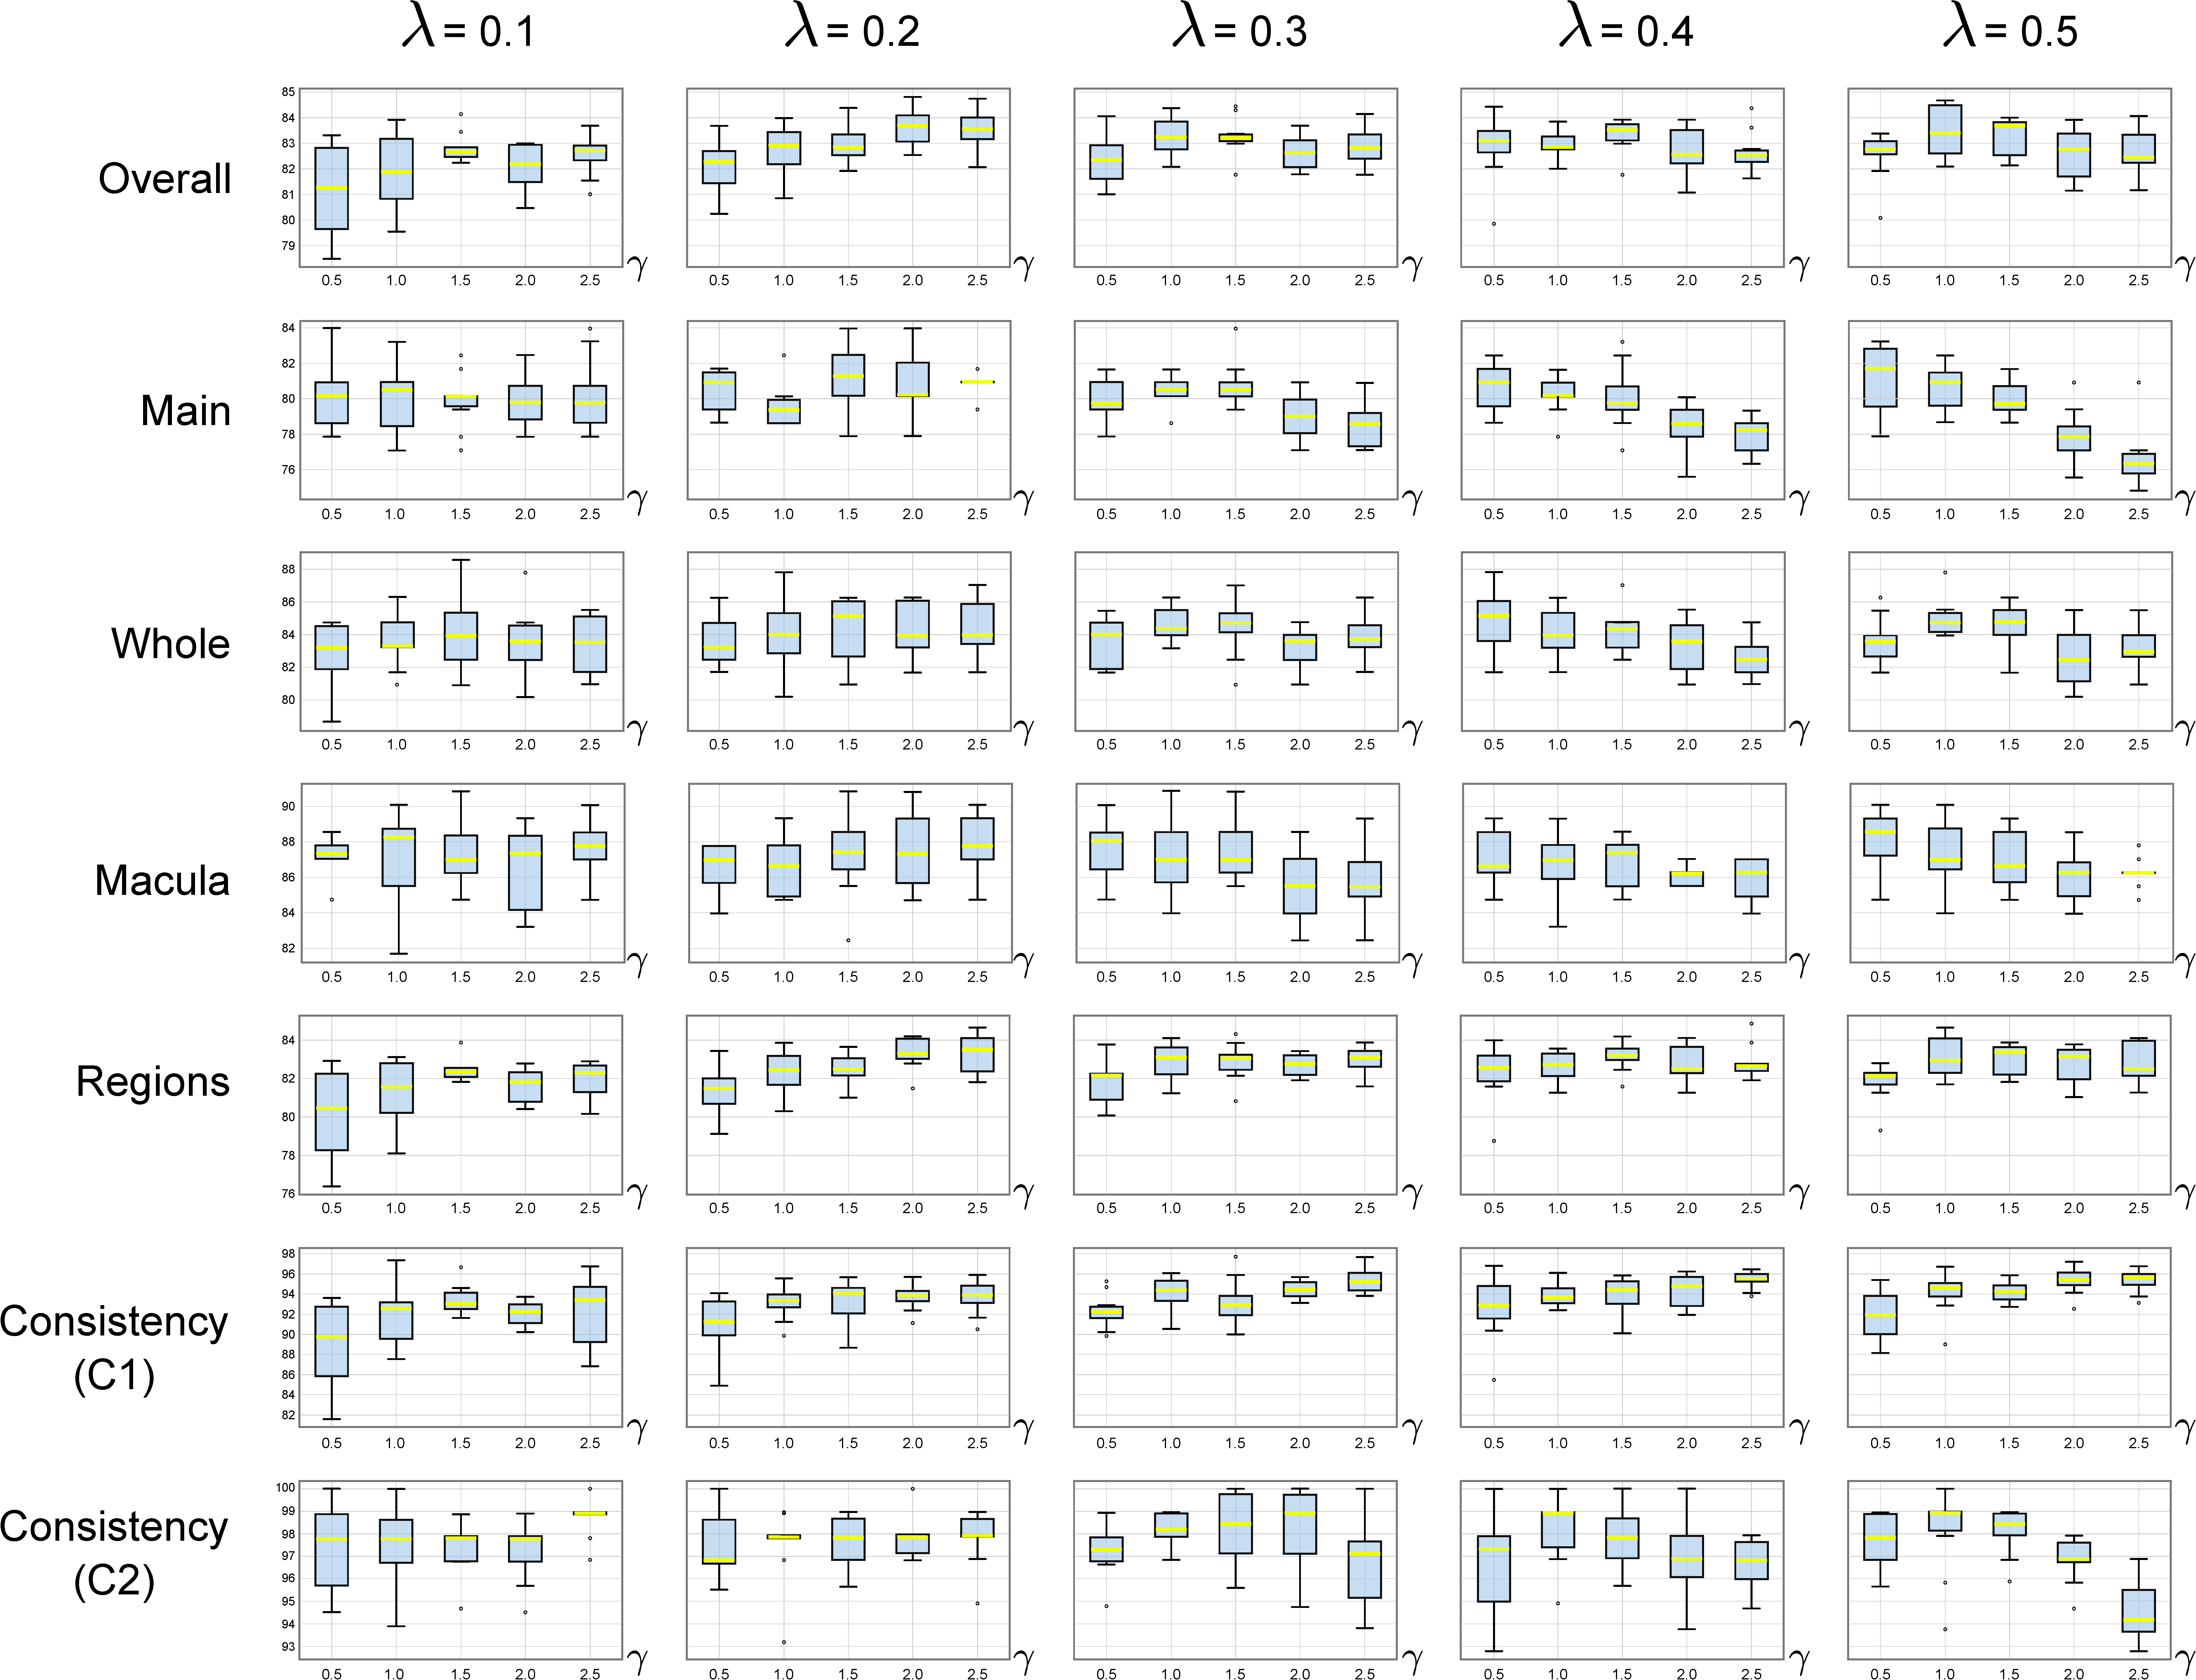
\includegraphics[width=\textwidth]{Figures/Part2_Consist/01_mainsub/boxplots.pdf}
\caption{Effect of the variation of the hyperparameters $\lambda$ and $\gamma$, for each metric. The first 5 rows refer to accuracy for all questions (overall), for main questions (main) and for sub-questions (whole, macula and regions). The last two rows correspond to the consistency. In general, a higher value of $\lambda$ leads to a higher consistency, which is the expected behavior. High values of both parameters can produce a decrease in the accuracy of main questions.}
\label{fig:supp_boxplots}
\end{center}
\end{figure}

\begin{figure}[!t]
\begin{center}
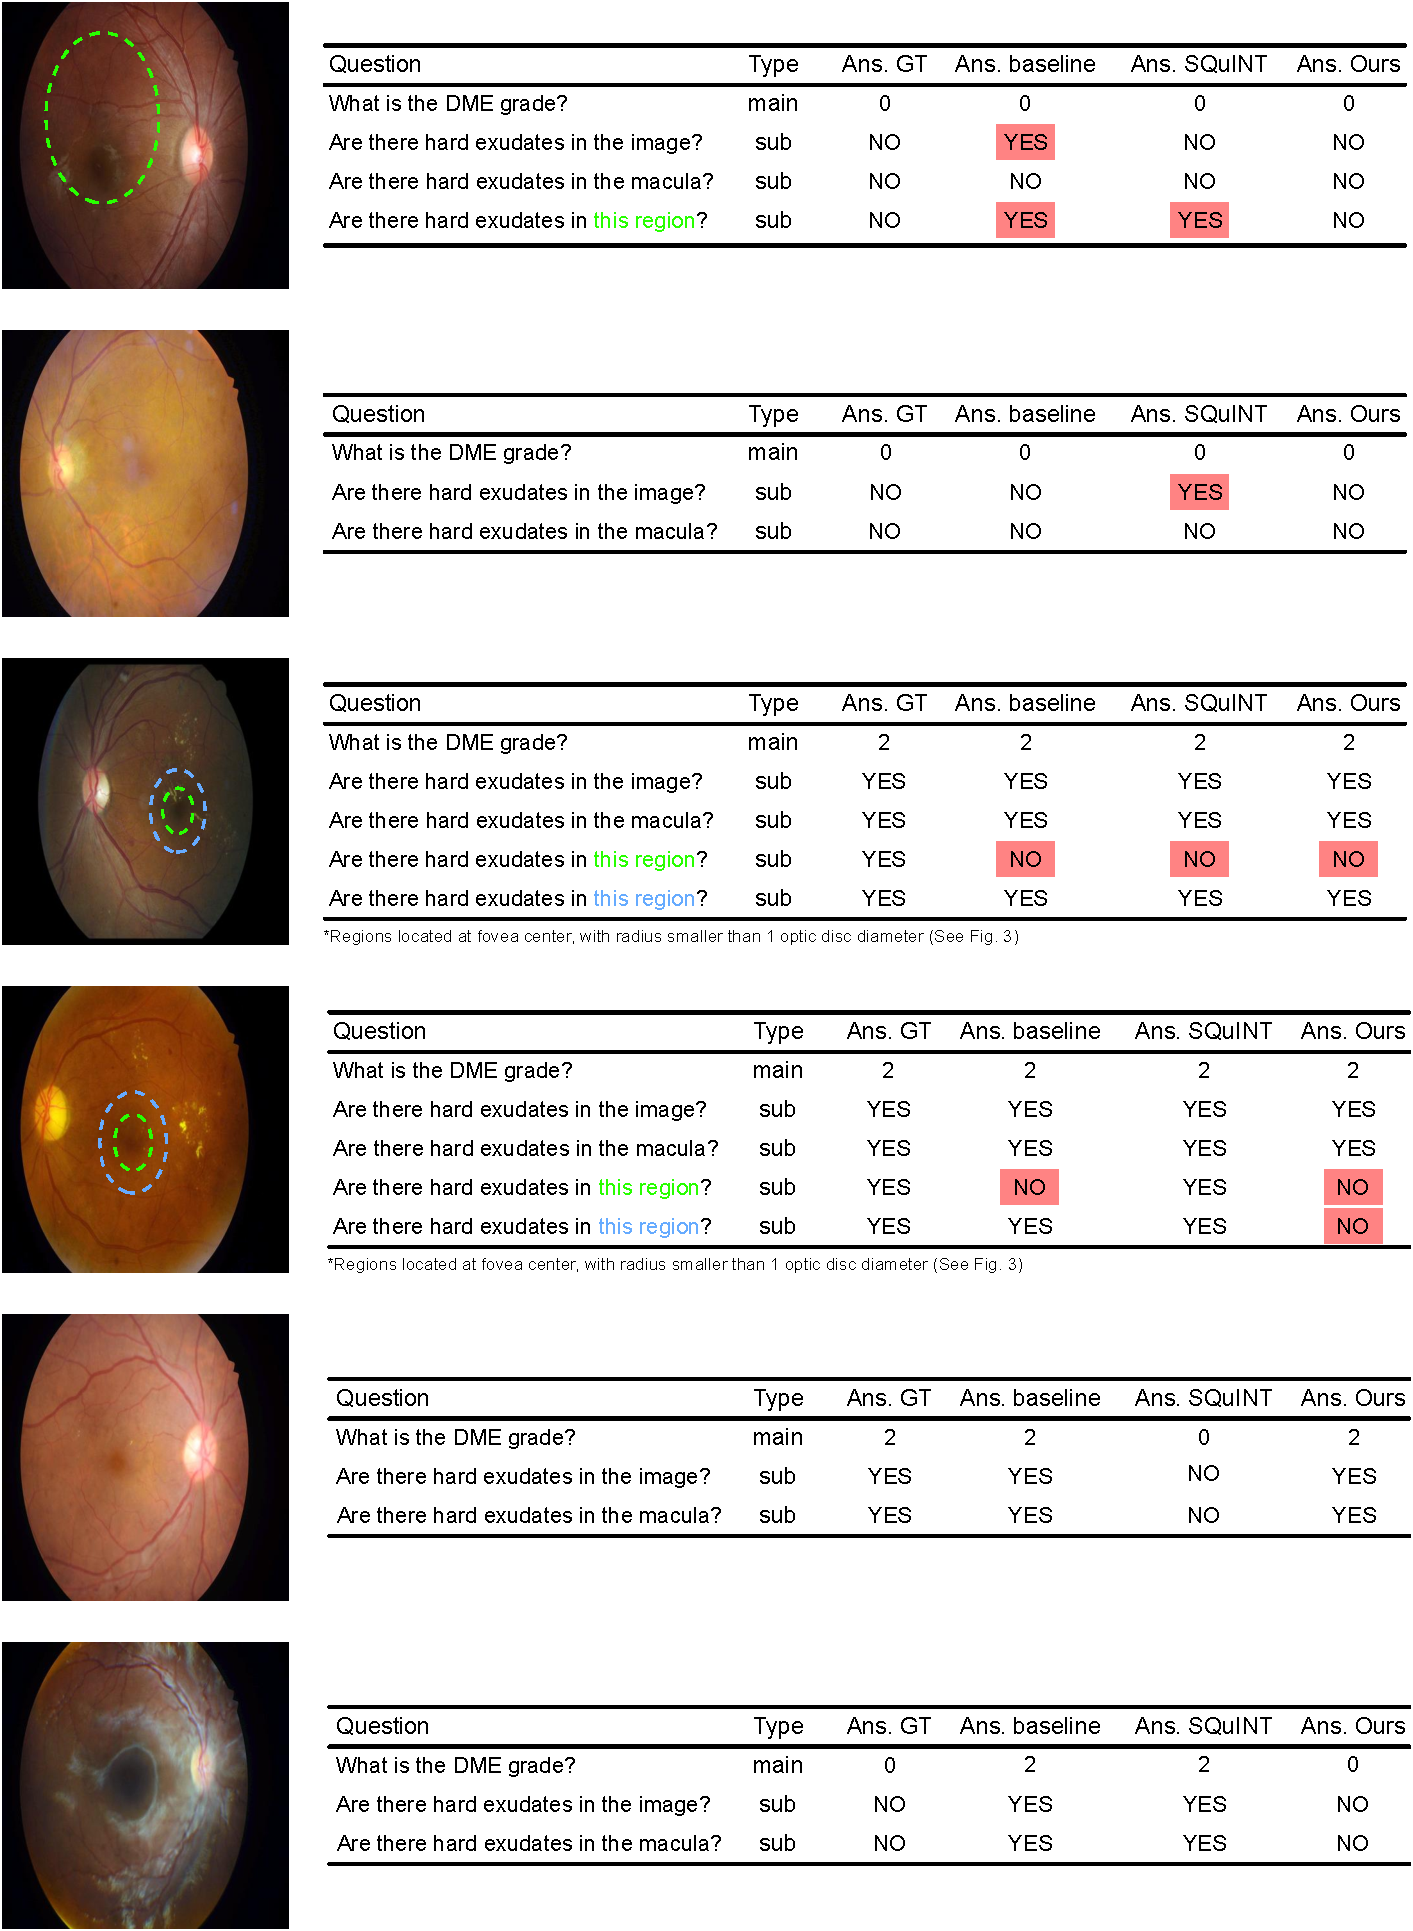
\includegraphics[width=\textwidth]{Figures/Part2_Consist/01_mainsub/examples_supplementary_ext.pdf}
\caption{Additional qualitative examples from the DME dataset. Inconsistent answers are highlighted in red. A more consistent behavior is observed in our method in comparison to the baselines (rows 1-2). Even though our method can make mistakes (rows 3-4), it also shows an improvement in the performance on main questions (rows 5-6).}
\label{fig:supp_examples}
\end{center}
\end{figure}